\chapter{Especificação do Sistema}
\label{chap:specification}

Este capítulo apresenta a especificação completa da
Medicano, abrangendo o levantamento de requisitos,
os requisitos funcionais e não-funcionais, os casos
de uso, as regras de negócio, a modelagem de dados
e a prototipação das telas.

\section{Levantamento de Requisitos}
\label{sec:requirements-gathering}

O levantamento de requisitos da Medicano foi realizado
por meio de análise de mercado, estudo de plataformas
concorrentes e discussões internas da equipe sobre
as necessidades dos perfis de usuário identificados
\cite{sommerville2011}. O sistema contempla quatro
perfis distintos com telas e fluxos próprios.

O \textbf{Paciente} é o usuário final da plataforma.
Busca profissionais e estabelecimentos de saúde por
especialidade e localização, utiliza o chatbot de
orientação para identificar a especialidade adequada
e realiza o agendamento de atendimentos. O paciente
não possui plano de assinatura no MVP.

O \textbf{Estabelecimento de Saúde} ou grupo de saúde é uma pessoa
jurídica que oferece serviços de saúde por meio de
múltiplos profissionais. Gerencia os profissionais
vinculados, configura os horários de atendimento e
acompanha os agendamentos pelo painel do funcionário
do estabelecimento de saúde (ou atendente). O acesso do funcionário
do estabelecimento de saúde (ou atendente) é realizado por meio de
login próprio vinculado à conta do estabelecimento de saúde. O Estabelecimento de Saúde
acessa a plataforma por meio de um plano de assinatura
do tipo grupo de saúde.

O \textbf{Autônomo de Saúde} é um profissional
independente --- como nutricionista, dentista, fisioterapeuta,
fonoaudiólogo, psicólogo ou profissional de saúde sem
estabelecimento de saúde vinculado --- que
oferece seus serviços diretamente pela plataforma.
Gerencia sua própria agenda e disponibilidade, sem
a possibilidade de delegar tarefas a outros usuários.
O autônomo acessa a plataforma por meio de um plano
de assinatura individual, com recursos proporcionais
ao plano contratado. A evolução para planos superiores
é possível dentro do próprio perfil.

O \textbf{Funcionário do estabelecimento de saúde (ou atendente)} é
um usuário vinculado a um estabelecimento de saúde, com login próprio
e acesso restrito às funcionalidades operacionais do
dia a dia: visualizar e gerenciar agendamentos,
confirmar ou cancelar consultas e administrar a agenda
dos profissionais do estabelecimento de saúde. O funcionário do estabelecimento de saúde
(ou atendente) não tem acesso às configurações da
conta, dados financeiros ou gestão de profissionais.

A Tabela~\ref{tab:profiles} resume os perfis e suas
principais características.

\begin{table}[H]
  \centering
  \caption{Perfis de usuário do sistema}
  \label{tab:profiles}
  \begin{tabular}{p{2.8cm}p{3cm}p{3cm}p{2.8cm}}
    \toprule
    \textbf{Perfil} &
    \textbf{Tipo} &
    \textbf{Plano} &
    \textbf{Delega tarefas} \\
    \midrule
    Paciente
      & Usuário final
      & Sem assinatura
      & Não \\
    Estabelecimento de Saúde
      & Pessoa jurídica
      & Grupo de saúde
      & Sim (atendente) \\
    Autônomo
      & Profissional independente
      & Individual
      & Não \\
    Funcionário (atendente)
      & Vinculado ao estabelecimento de saúde
      & Incluso no plano
      & Não \\
    \bottomrule
  \end{tabular}
  \fonte{Elaborado pelos autores (2026)}
\end{table}

\section{Requisitos Funcionais}
\label{sec:functional-requirements}

Os requisitos funcionais descrevem o comportamento
esperado do sistema para cada perfil de usuário
\cite{sommerville2011}. As tabelas a seguir
apresentam os requisitos organizados por perfil.

\subsection{Requisitos do Paciente}
\label{subsec:patient-requirements}

\begin{table}[H]
  \centering
  \caption{Requisitos funcionais --- Paciente}
  \label{tab:patient-requirements}
  \begin{tabular}{p{1.2cm}p{6.5cm}p{2.5cm}}
    \toprule
    \textbf{ID} &
    \textbf{Descrição} &
    \textbf{Prioridade} \\
    \midrule
    RF01 & O sistema deve permitir o cadastro de
           pacientes com nome, e-mail, senha,
           data de nascimento e telefone celular;
           opcionalmente gênero, pronomes,
           CEP, cidade e estado
         & Alta \\
    RF02 & O sistema deve permitir o login de
           pacientes com e-mail e senha
         & Alta \\
    RF03 & O sistema deve permitir ao paciente
           iniciar uma conversa de orientação com
           o chatbot para identificar a
           especialidade adequada às suas
           necessidades
         & Alta \\
    RF04 & O sistema deve redirecionar o paciente
           para a busca filtrada pela especialidade
           identificada ao final da orientação
         & Alta \\
    RF05 & O sistema deve permitir a busca de
           estabelecimentos de saúde e profissionais autônomos
           por especialidade e cidade
         & Alta \\
    RF06 & O sistema deve exibir o perfil público
           de estabelecimentos de saúde e profissionais, incluindo
           especialidades, endereço e horários
           disponíveis
         & Alta \\
    RF07 & O sistema deve permitir ao paciente
           agendar atendimento diretamente com
           um profissional autônomo
         & Alta \\
    RF08 & O sistema deve permitir ao paciente
           agendar atendimento com um estabelecimento de saúde
           escolhendo um profissional específico
           dentre os disponíveis
         & Alta \\
    RF09 & O sistema deve permitir ao paciente
           agendar atendimento com um estabelecimento de saúde
           sem especificar o profissional,
           deixando a alocação a critério
           do estabelecimento de saúde
         & Alta \\
    RF10 & O sistema deve exibir ao paciente o
           status do agendamento: pendente,
           confirmado ou cancelado
         & Alta \\
    RF11 & O sistema deve permitir ao paciente
           visualizar seu histórico de
           agendamentos
         & Alta \\
    RF12 & O sistema deve permitir ao paciente
           cancelar um agendamento respeitando
           as regras de antecedência definidas
           pelo prestador
         & Média \\
    RF13 & O sistema deve permitir ao paciente
           editar seus dados cadastrais
         & Média \\
    \bottomrule
  \end{tabular}
  \fonte{Elaborado pelos autores (2026)}
\end{table}

\subsection{Requisitos do estabelecimento de saúde}
\label{subsec:clinic-requirements}

\begin{table}[H]
  \centering
  \caption{Requisitos funcionais --- Estabelecimento de Saúde}
  \label{tab:clinic-requirements}
  \begin{tabular}{p{1.2cm}p{6.5cm}p{2.5cm}}
    \toprule
    \textbf{ID} &
    \textbf{Descrição} &
    \textbf{Prioridade} \\
    \midrule
    RF14 & O sistema deve permitir o cadastro de
           estabelecimentos de saúde com razão social, CNPJ,
           endereço e especialidades oferecidas
         & Alta \\
    RF15 & O sistema deve permitir ao estabelecimento de saúde
           selecionar e ativar um plano de
           assinatura do tipo grupo de saúde
         & Alta \\
    RF16 & O sistema deve permitir ao estabelecimento de saúde
           cadastrar e gerenciar profissionais
           de saúde vinculados à sua conta
         & Alta \\
    RF17 & O sistema deve permitir ao estabelecimento de saúde
           cadastrar funcionários (ou atendentes)
           com login próprio e acesso restrito
           às funcionalidades operacionais
         & Alta \\
    RF18 & O sistema deve permitir ao estabelecimento de saúde
           configurar os slots de disponibilidade
           por profissional, dia da semana
           e horário
         & Alta \\
    RF19 & O sistema deve permitir ao estabelecimento de saúde
           configurar se os agendamentos são
           confirmados automaticamente ou
           manualmente
         & Alta \\
    RF20 & O sistema deve permitir ao estabelecimento de saúde
           visualizar a agenda do dia e da
           semana por profissional
         & Alta \\
    RF21 & O sistema deve permitir ao estabelecimento de saúde
           criar agendamentos manualmente pelo
           painel do funcionário (ou atendente)
         & Alta \\
    RF22 & O sistema deve permitir ao estabelecimento de saúde
           confirmar, recusar ou cancelar
           agendamentos
         & Alta \\
    RF23 & O sistema deve permitir ao estabelecimento de saúde
           definir o tempo mínimo de antecedência
           para cancelamento pelo paciente
         & Média \\
    RF24 & O sistema deve permitir ao estabelecimento de saúde
           editar seu perfil, endereço e
           especialidades
         & Média \\
    RF25 & O sistema deve permitir ao estabelecimento de saúde
           configurar a conexão de agendamento
           entre funcionários, habilitando
           consultas consecutivas sem intervalo
           mínimo
         & Média \\
    \bottomrule
  \end{tabular}
  \fonte{Elaborado pelos autores (2026)}
\end{table}

\subsection{Requisitos do Autônomo de Saúde}
\label{subsec:professional-requirements}

\begin{table}[H]
  \centering
  \caption{Requisitos funcionais --- Autônomo de saúde}
  \label{tab:professional-requirements}
  \begin{tabular}{p{1.2cm}p{6.5cm}p{2.5cm}}
    \toprule
    \textbf{ID} &
    \textbf{Descrição} &
    \textbf{Prioridade} \\
    \midrule
    RF26 & O sistema deve permitir o cadastro de
           autônomos com nome, CPF, especialidade,
           registro profissional e endereço de
           atendimento
         & Alta \\
    RF27 & O sistema deve permitir ao autônomo
           selecionar e ativar um plano de
           assinatura individual
         & Alta \\
    RF28 & O sistema deve permitir ao autônomo
           configurar seus slots de disponibilidade
           por dia da semana e horário
         & Alta \\
    RF29 & O sistema deve permitir ao autônomo
           configurar se os agendamentos são
           confirmados automaticamente ou
           manualmente
         & Alta \\
    RF30 & O sistema deve permitir ao autônomo
           configurar o tempo mínimo de
           antecedência para agendamento
         & Alta \\
    RF31 & O sistema deve permitir ao autônomo
           visualizar sua agenda do dia e
           da semana
         & Alta \\
    RF32 & O sistema deve permitir ao autônomo
           criar agendamentos manualmente
           pelo seu painel
         & Alta \\
    RF33 & O sistema deve permitir ao autônomo
           confirmar, recusar ou cancelar
           agendamentos
         & Alta \\
    RF34 & O sistema deve permitir ao autônomo
           definir o tempo mínimo de antecedência
           para cancelamento pelo paciente
         & Média \\
    RF35 & O sistema deve permitir ao autônomo
           editar seu perfil e especialidade
         & Média \\
    RF36 & O sistema deve permitir ao autônomo
           realizar upgrade de plano de
           assinatura pelo próprio painel
         & Média \\
    \bottomrule
  \end{tabular}
  \fonte{Elaborado pelos autores (2026)}
\end{table}

\subsection{Requisitos do Funcionário do estabelecimento de saúde}
\label{subsec:attendant-requirements}

\begin{table}[H]
  \centering
  \caption{Requisitos funcionais --- Funcionário do estabelecimento de saúde (ou atendente)}
  \label{tab:attendant-requirements}
  \begin{tabular}{p{1.2cm}p{6.5cm}p{2.5cm}}
    \toprule
    \textbf{ID} &
    \textbf{Descrição} &
    \textbf{Prioridade} \\
    \midrule
    RF37 & O sistema deve permitir ao funcionário
           (ou atendente) fazer login com nome de
           usuário e senha, sem necessidade de
           e-mail, utilizando credenciais criadas
           pelo estabelecimento de saúde à qual está vinculado
         & Alta \\
    RF38 & O sistema deve permitir ao funcionário
           (ou atendente) visualizar a agenda do
           dia e da semana de todos os
           profissionais do estabelecimento de saúde
         & Alta \\
    RF39 & O sistema deve permitir ao funcionário
           (ou atendente) criar agendamentos
           manualmente para qualquer profissional
           do estabelecimento de saúde
         & Alta \\
    RF40 & O sistema deve permitir ao funcionário
           (ou atendente) confirmar, recusar ou
           cancelar agendamentos
         & Alta \\
    RF41 & O sistema deve impedir o funcionário
           (ou atendente) de acessar configurações
           da conta, dados financeiros e gestão
           de profissionais
         & Alta \\
    \bottomrule
  \end{tabular}
  \fonte{Elaborado pelos autores (2026)}
\end{table}

\subsection{Requisitos do Sistema de Assinaturas}
\label{subsec:subscription-requirements}

\begin{table}[H]
  \centering
  \caption{Requisitos funcionais --- Assinaturas}
  \label{tab:subscription-requirements}
  \begin{tabular}{p{1.2cm}p{6.5cm}p{2.5cm}}
    \toprule
    \textbf{ID} &
    \textbf{Descrição} &
    \textbf{Prioridade} \\
    \midrule
    RF42 & O sistema deve oferecer um plano
           individual destinado ao autônomo
           de saúde, com funcionalidades
           proporcionais ao plano contratado
         & Alta \\
    RF43 & O sistema deve oferecer um plano
           grupo de saúde destinado aos estabelecimentos de saúde,
           com suporte a múltiplos profissionais
           e funcionários (ou atendentes)
         & Alta \\
    RF44 & O sistema deve restringir
           funcionalidades avançadas a usuários
           sem plano ativo ou com plano expirado
         & Alta \\
    RF45 & O sistema deve permitir ao autônomo
           realizar upgrade de plano pelo
           próprio painel sem suporte externo
         & Média \\
    RF46 & O paciente não possui plano de
           assinatura e acessa todas as
           funcionalidades de busca e
           agendamento gratuitamente
         & Alta \\
    \bottomrule
  \end{tabular}
  \fonte{Elaborado pelos autores (2026)}
\end{table}

\section{Requisitos Não-Funcionais}
\label{sec:non-functional-requirements}

Os requisitos não-funcionais definem as qualidades
que o sistema deve apresentar, independentemente
das funcionalidades específicas \cite{sommerville2011}.

\begin{table}[H]
  \centering
  \caption{Requisitos não-funcionais}
  \label{tab:non-functional-requirements}
  \begin{tabular}{p{1.2cm}p{3.8cm}p{6.2cm}}
    \toprule
    \textbf{ID} &
    \textbf{Categoria} &
    \textbf{Descrição} \\
    \midrule
    RNF01 & Desempenho
          & Os endpoints da API devem responder
            em menos de 500ms para o percentil
            95 das requisições \\
    RNF02 & Disponibilidade
          & O sistema deve ter disponibilidade
            mínima de 99\% medida mensalmente \\
    RNF03 & Segurança
          & Toda comunicação entre cliente e
            servidor deve ser realizada via
            HTTPS com TLS 1.3 \\
    RNF04 & Segurança
          & Senhas devem ser armazenadas com
            hash Bcrypt com fator de custo
            mínimo de 12 \cite{provos1999} \\
    RNF05 & Segurança
          & Tokens JWT devem ter expiração de
            7 dias e ser revogáveis via Redis
            \cite{rfc7519} \\
    RNF06 & Segurança
          & Credenciais e segredos não devem
            ser armazenados no código-fonte
            ou em arquivos versionados \\
    RNF07 & Conformidade
          & O sistema deve estar em conformidade
            com a LGPD no tratamento de dados
            pessoais e sensíveis dos usuários
            \cite{lgpd2018} \\
    RNF08 & Conformidade
          & O chatbot de orientação deve exibir
            aviso de que suas recomendações não
            substituem avaliação profissional,
            em conformidade com a Resolução
            CFM n.º 2.336/2023 \cite{cfm23362023} \\
    RNF09 & Manutenibilidade
          & O código deve seguir os padrões
            definidos pelo ESLint e Prettier
            configurados no repositório \\
    RNF10 & Manutenibilidade
          & A API deve ter documentação
            automática gerada via Swagger
            acessível em \texttt{/api/docs} \\
    RNF11 & Escalabilidade
          & A arquitetura deve permitir
            escalabilidade horizontal do
            backend sem alterações no código \\
    RNF12 & Usabilidade
          & O sistema deve ser responsivo e
            funcionar em dispositivos móveis
            e desktop \\
    \bottomrule
  \end{tabular}
  \fonte{Elaborado pelos autores (2026)}
\end{table}

\section{Casos de Uso}
\label{sec:use-cases}

Os casos de uso descrevem as interações entre os
atores e o sistema para realizar um objetivo
específico \cite{sommerville2011}. Os atores
principais são o Paciente, o Prestador de Serviço
--- que abrange tanto o estabelecimento de saúde quanto o Autônomo
de Saúde --- o Funcionário do estabelecimento de saúde (ou atendente),
o Visitante --- usuário não autenticado que navega
pela plataforma --- e o Sistema, que representa os
processos automatizados.

\subsection{UC01 --- Orientação e Agendamento pelo Paciente}
\label{subsec:uc01}

\begin{table}[H]
  \centering
  \caption{UC01 --- Orientação e agendamento pelo paciente}
  \label{tab:uc01}
  \begin{tabular}{p{3cm}p{8.5cm}}
    \toprule
    \textbf{Elemento} & \textbf{Descrição} \\
    \midrule
    Ator principal  & Paciente \\
    Pré-condição    & Paciente autenticado no sistema \\
    Fluxo principal &
      1. Paciente acessa o chatbot de orientação \newline
      2. Chatbot conduz conversa sobre sintomas \newline
      3. Chatbot recomenda especialidade e redireciona
         para busca filtrada \newline
      4. Paciente seleciono estabelecimento de saúde ou autônomo \newline
      5. Se selecionou estabelecimento de saúde: paciente pode escolher
         um profissional específico ou deixar a
         critério do estabelecimento de saúde \newline
      6. Paciente escolhe data e horário disponível \newline
      7. Sistema valida conflito de horários com
         agendamentos existentes do paciente \newline
      8. Sistema registra agendamento com status
         conforme configuração do prestador \newline
      9. Paciente recebe confirmação na tela \\
    Fluxo alternativo &
      3a. Paciente ignora orientação e busca
          diretamente por especialidade \newline
      7a. Se houver conflito de horário, sistema
          exibe mensagem e bloqueia o agendamento \newline
      8a. Se configuração for manual, status fica
          pendente até confirmação do prestador \\
    Pós-condição    & Agendamento registrado no sistema \\
    \bottomrule
  \end{tabular}
  \fonte{Elaborado pelos autores (2026)}
\end{table}

\subsection{UC02 --- Gestão de Agenda pelo Prestador}
\label{subsec:uc02}

\begin{table}[H]
  \centering
  \caption{UC02 --- Gestão de agenda pelo prestador}
  \label{tab:uc02}
  \begin{tabular}{p{3cm}p{8.5cm}}
    \toprule
    \textbf{Elemento} & \textbf{Descrição} \\
    \midrule
    Ator principal  & Estabelecimento de Saúde, Funcionário (atendente)
                      ou Autônomo \\
    Pré-condição    & Ator autenticado no sistema \\
    Fluxo principal &
      1. Ator acessa o dashboard de agenda \newline
      2. Sistema exibe agendamentos do dia e
         da semana \newline
      3. Ator visualiza agendamentos pendentes \newline
      4. Ator confirma ou recusa cada
         agendamento pendente \newline
      5. Sistema atualiza o status do agendamento \\
    Fluxo alternativo &
      1a. Prestador configura confirmação automática
          --- agendamentos já chegam confirmados,
          sem necessidade de ação manual \\
    Pós-condição    & Status do agendamento atualizado \\
    \bottomrule
  \end{tabular}
  \fonte{Elaborado pelos autores (2026)}
\end{table}

\subsection{UC03 --- Cancelamento de Agendamento}
\label{subsec:uc03}

\begin{table}[H]
  \centering
  \caption{UC03 --- Cancelamento de agendamento}
  \label{tab:uc03}
  \begin{tabular}{p{3cm}p{8.5cm}}
    \toprule
    \textbf{Elemento} & \textbf{Descrição} \\
    \midrule
    Atores          & Paciente, Prestador ou
                      Funcionário (atendente) \\
    Pré-condição    & Agendamento com status confirmado
                      ou pendente \\
    Fluxo --- Paciente &
      1. Paciente acessa seus agendamentos \newline
      2. Paciente solicita cancelamento \newline
      3. Sistema verifica se a antecedência mínima
         configurada pelo prestador foi respeitada \newline
      4. Se respeitada, agendamento é cancelado \newline
      5. Se não respeitada, sistema exibe mensagem
         informando o prazo mínimo \\
    Fluxo --- Prestador &
      1. Prestador ou funcionário (atendente)
         acessa o dashboard \newline
      2. Cancela o agendamento \newline
      3. Sistema cancela sem restrição de prazo \\
    Pós-condição    & Agendamento com status cancelado
                      e slot liberado na agenda \\
    \bottomrule
  \end{tabular}
  \fonte{Elaborado pelos autores (2026)}
\end{table}

\subsection{UC04 --- Busca Direta por Estabelecimento de Saúde ou Profissional}
\label{subsec:uc04}

\begin{table}[H]
  \centering
  \caption{UC04 --- Busca direta por estabelecimento de saúde ou profissional}
  \label{tab:uc04}
  \begin{tabular}{p{3cm}p{8.5cm}}
    \toprule
    \textbf{Elemento} & \textbf{Descrição} \\
    \midrule
    Ator principal  & Visitante (autenticado ou não) \\
    Pré-condição    & Nenhuma --- acesso público sem
                      necessidade de login \\
    Fluxo principal &
      1. Visitante acessa \texttt{/buscar} \newline
      2. Visitante aplica filtros de especialidade
         e cidade \newline
      3. Sistema exibe lista de estabelecimentos de saúde e
         profissionais disponíveis \newline
      4. Visitante seleciona um resultado e
         visualiza o perfil completo \newline
      5. Visitante visualiza horários disponíveis \\
    Fluxo alternativo &
      5a. Visitante decide agendar --- se não
          autenticado, é redirecionado para
          \texttt{/login} com retorno automático
          ao perfil após autenticação \newline
      5b. Visitante decide não agendar e
          encerra a navegação \\
    Pós-condição    & Nenhuma --- fluxo de leitura
                      sem alteração de estado \\
    \bottomrule
  \end{tabular}
  \fonte{Elaborado pelos autores (2026)}
\end{table}

\section{Regras de Negócio}
\label{sec:business-rules}

As regras de negócio definem as restrições e
políticas que governam o comportamento do sistema
independentemente da interface ou tecnologia
utilizada \cite{martin2017}.

\begin{center}
\small
\begin{longtable}{p{1.2cm}p{3cm}p{7.5cm}}
  \caption{Regras de negócio}
  \label{tab:business-rules} \\
  \toprule
  \textbf{ID} &
  \textbf{Contexto} &
  \textbf{Regra} \\
  \midrule
  \endfirsthead

  \multicolumn{3}{l}{\small\itshape continuação da página anterior} \\
  \toprule
  \textbf{ID} &
  \textbf{Contexto} &
  \textbf{Regra} \\
  \midrule
  \endhead

  \midrule
  \multicolumn{3}{r}{\small\itshape continua na próxima página} \\
  \endfoot

  \bottomrule
  \multicolumn{3}{r}{\small Fonte: Elaborado pelos autores (2026)} \\
  \endlastfoot

  RN01 & Agendamento
      & Um paciente não pode ter dois
        agendamentos com horários
        sobrepostos, independentemente
        do prestador ou estabelecimento de saúde \\
  RN02 & Agendamento
      & Consultas consecutivas com o mesmo
        prestador são permitidas sem
        intervalo mínimo obrigatório \\
  RN03 & Agendamento
      & Consultas com prestadores diferentes
        da mesmo estabelecimento de saúde podem ser agendadas
        consecutivamente se o estabelecimento de saúde tiver
        habilitado a conexão de agendamento
        entre funcionários \\
  RN04 & Agendamento
      & Consultas com prestadores de estabelecimentos de saúde
        diferentes exigem intervalo mínimo
        de 30 minutos entre os horários \\
  RN05 & Agendamento
      & O tempo mínimo de antecedência para
        agendamento é configurável pelo
        prestador, podendo ser definido
        em horas ou minutos \\
  RN06 & Agendamento
      & O status inicial do agendamento é
        definido pela configuração do
        prestador: \textit{confirmado} se
        automático ou \textit{pendente}
        se manual \\
  RN07 & Agendamento
      & Um slot ocupado não pode ser
        agendado por outro paciente enquanto
        estiver com status pendente ou
        confirmado \\
  RN08 & Cancelamento
      & O paciente só pode cancelar com
        antecedência mínima definida pelo
        prestador, que pode ser de 0 a
        72 horas \\
  RN09 & Cancelamento
      & O prestador pode cancelar um
        agendamento a qualquer momento,
        sem restrição de prazo \\
  RN10 & Cancelamento
      & Ao cancelar um agendamento, o slot
        correspondente é automaticamente
        liberado na agenda \\
  RN11 & Perfis
      & O tipo de conta de um usuário é
        definido no momento do cadastro
        e não pode ser alterado
        posteriormente \\
  RN12 & Perfis
      & Contas cadastradas como prestador
        de serviço --- estabelecimento de saúde ou autônomo
        --- não podem ser convertidas para
        conta de paciente \\
  RN13 & Perfis
      & É permitido realizar upgrade do
        plano individual (autônomo) para
        o plano grupo de saúde (estabelecimento de saúde),
        mas não o inverso \\
  RN14 & Perfis
      & Um Estabelecimento de Saúde pode ter múltiplos
        profissionais e funcionários
        (ou atendentes) vinculados
        à sua conta \\
  RN15 & Perfis
      & Um autônomo de saúde não pode estar
        vinculado a um estabelecimento de saúde no sistema
        --- são perfis independentes \\
  RN16 & Chatbot
      & O chatbot deve exibir aviso de
        isenção de responsabilidade
        diagnóstica no início de cada
        conversa \cite{cfm23362023,masanneck2024} \\
  RN17 & Chatbot
      & O chatbot deve recomendar no máximo
        uma especialidade por conversa de
        orientação e redirecionar para a busca
        filtrada ao final \cite{masanneck2024} \\
  RN18 & Autenticação
      & O token JWT é invalidado
        imediatamente no logout,
        independentemente do seu prazo
        de expiração \cite{rfc7519} \\
  RN19 & Autenticação
      & Sessões expiram automaticamente
        após 7 dias de inatividade \\
  RN20 & Assinaturas
      & O autônomo sem plano ativo não
        aparece nos resultados de busca
        da plataforma \\
  RN21 & Assinaturas
      & O funcionário (ou atendente) só
        pode ser cadastrado se o estabelecimento de saúde
        possuir plano grupo de saúde ativo \\
  RN22 & Assinaturas
      & O downgrade de plano não é
        permitido enquanto houver
        agendamentos futuros confirmados \\
  RN23 & Funcionário
      & Um funcionário (ou atendente) está
        sempre vinculado a uma único estabelecimento de saúde
        e não pode acessar dados de outras
        estabelecimentos de saúde \\
  RN24 & Agendamento
      & Quando o paciente não especifica o
        profissional ao agendar com uma
        estabelecimento de saúde, a alocação fica a critério
        do estabelecimento de saúde e pode ser definida pelo
        funcionário (ou atendente) no painel \\
  RN25 & Agendamento
      & A conexão de agendamento entre
        funcionários da mesmo estabelecimento de saúde ---
        que permite consultas consecutivas
        sem intervalo --- é configurável
        pelo gestor do estabelecimento de saúde e está
        desabilitada por padrão \\
  RN26 & Autenticação
      & O funcionário (ou atendente) autentica-se
        exclusivamente por nome de usuário e senha,
        sem e-mail associado à conta \\
  RN27 & Autenticação
      & O nome de usuário do funcionário (ou
        atendente) deve ser único dentro do
        escopo do estabelecimento de saúde à qual está vinculado,
        podendo existir o mesmo nome de usuário
        em estabelecimentos de saúde diferentes \\
  \end{longtable}
\end{center}

\section{Modelagem de Dados}
\label{sec:data-modeling}

A modelagem de dados da Medicano é baseada no
modelo orientado a documentos do MongoDB, no qual
cada registro é armazenado como um documento
autônomo que pode conter campos aninhados e
arrays sem necessidade de esquema rígido
\cite{sadalage2012}. Essa abordagem é
particularmente adequada para domínios cujos
objetos possuem estrutura variável entre
instâncias --- como os diferentes perfis de
usuário da plataforma \cite{fowler2012nosql}.
A Figura~\ref{fig:der} apresenta a visão geral das
entidades e seus relacionamentos; as principais
entidades do sistema são descritas em detalhe a
seguir.

\begin{figure}[H]
  \centering
  \caption{Diagrama entidade-relacionamento da Medicano}
  \label{fig:der}
  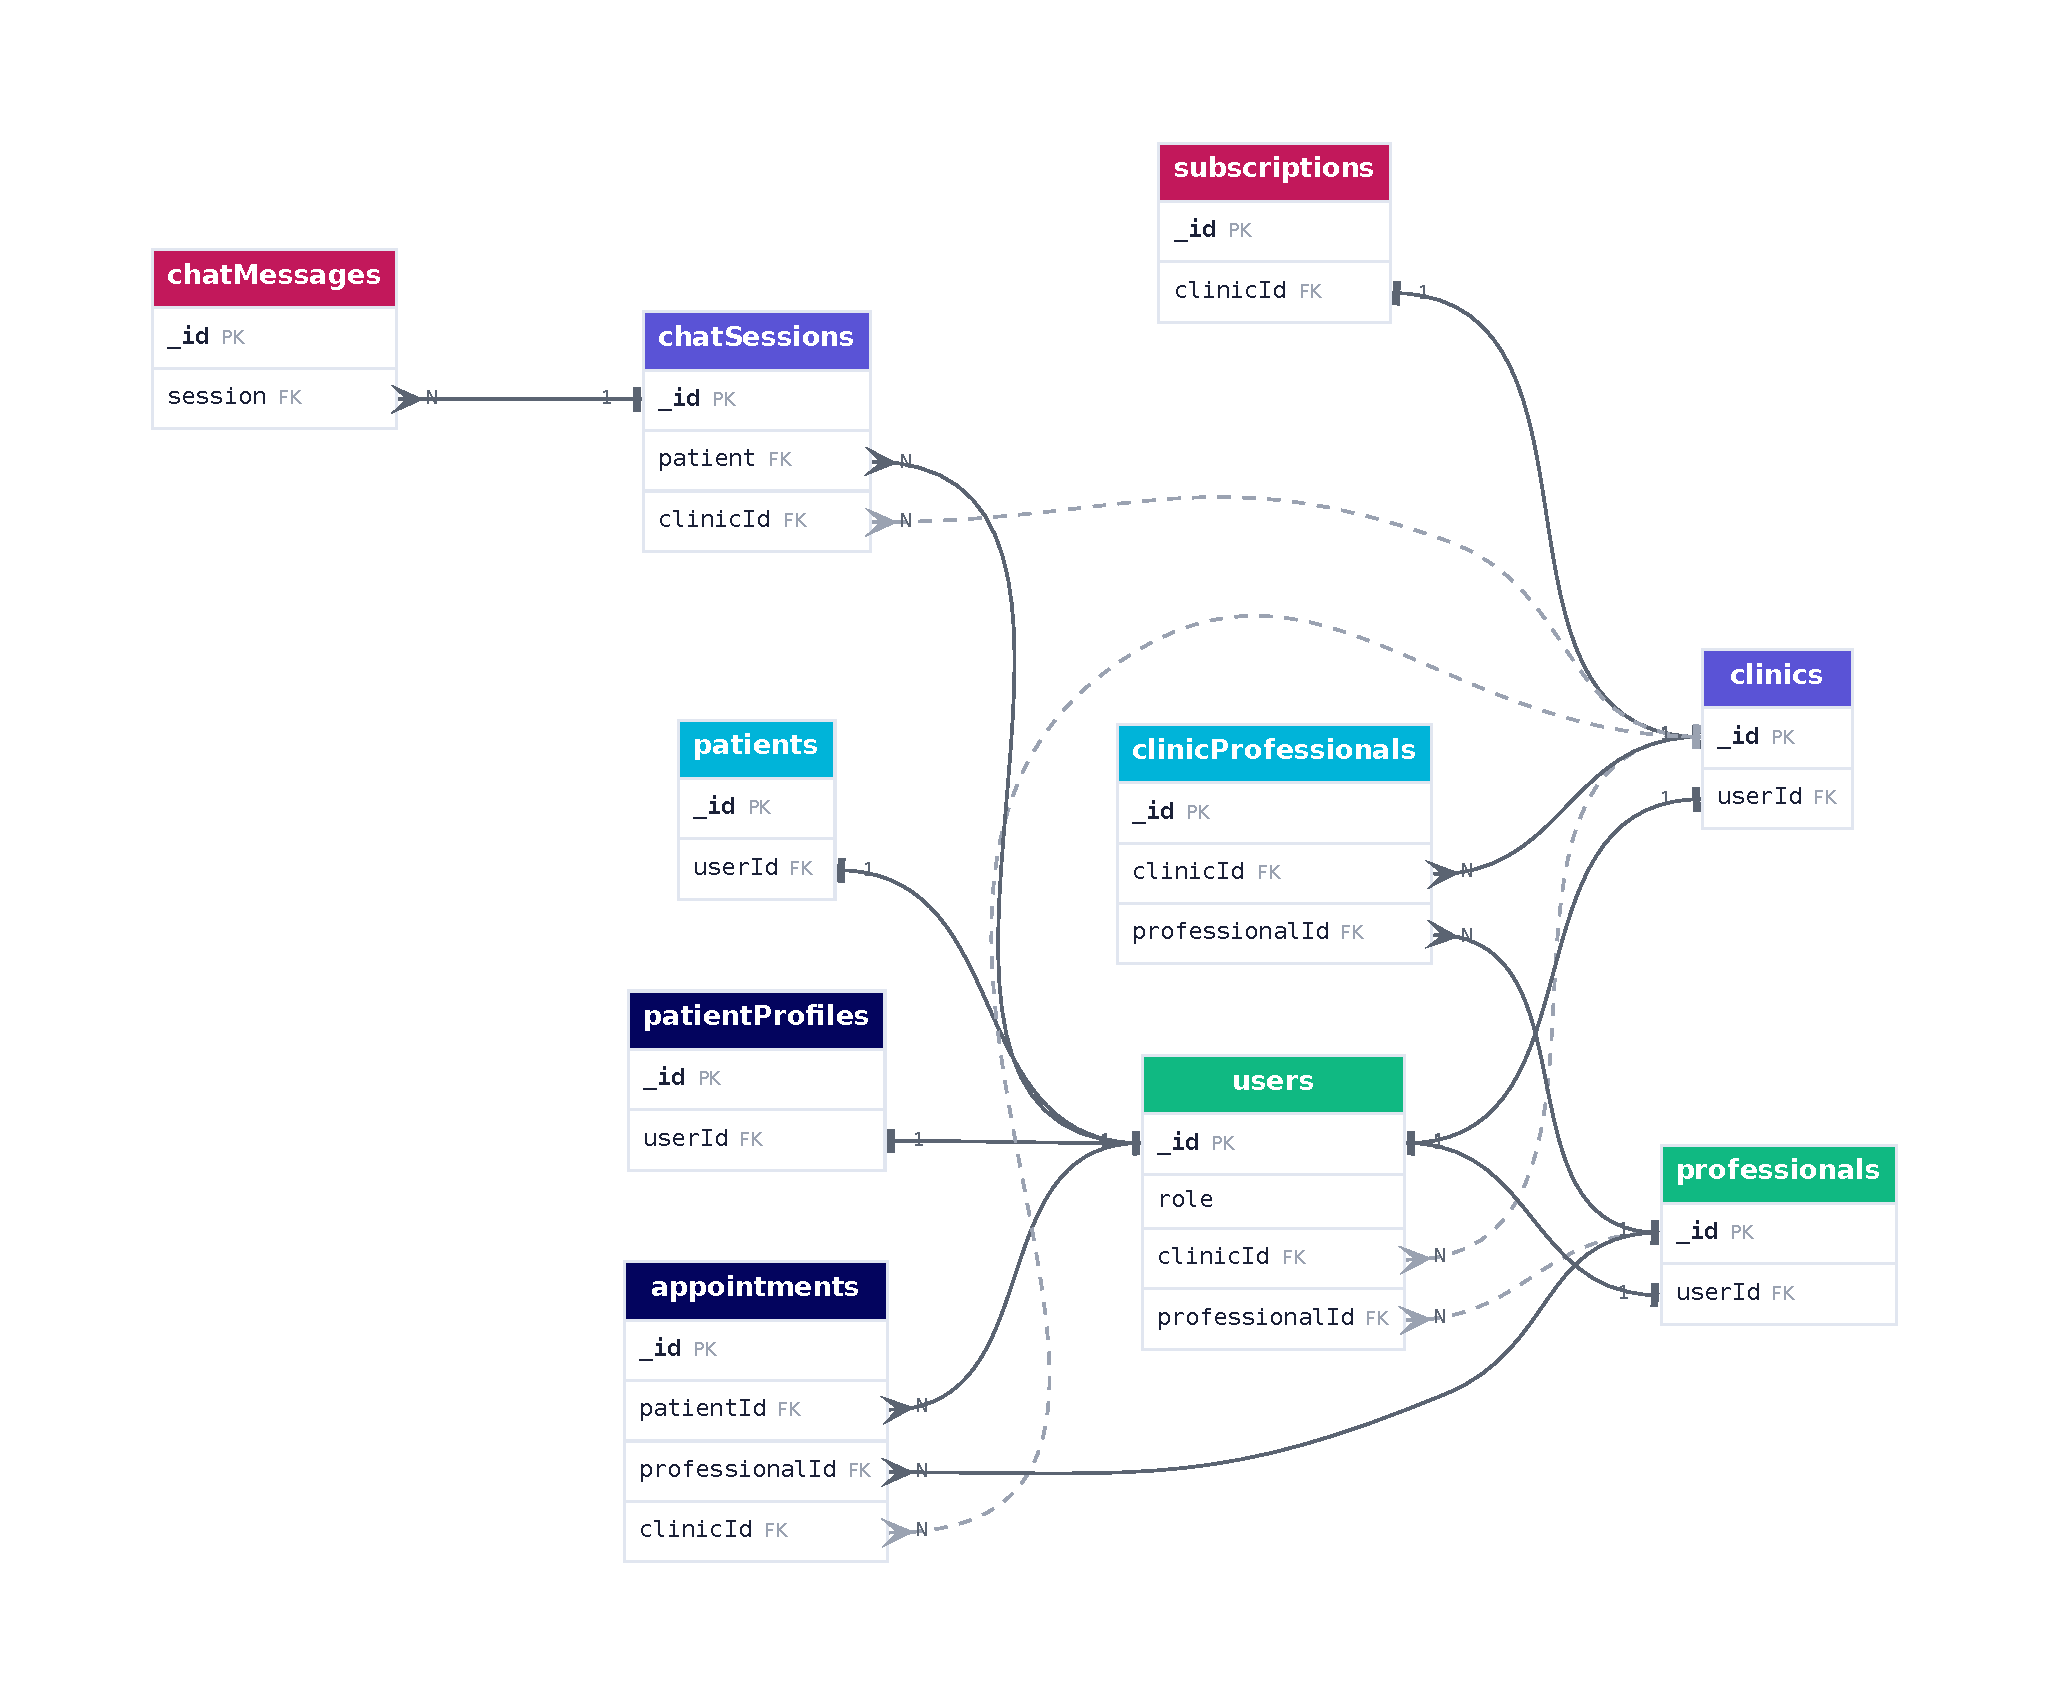
\includegraphics[width=0.95\textwidth]
    {assets/diagrams/Medicano_DER}
  \fonte{Elaborado pelos autores (2026)}
\end{figure}

\subsection{Entidade User}
\label{subsec:entity-user}

Representa todos os usuários do sistema,
independentemente do perfil. O campo \texttt{role}
determina o tipo de acesso e os fluxos disponíveis.
Contas do tipo \texttt{attendant} utilizam nome de
usuário para autenticação, dispensando e-mail, pois
são criadas e gerenciadas diretamente pelo estabelecimento de saúde
à qual estão vinculados.

\begin{table}[H]
  \centering
  \caption{Entidade User}
  \label{tab:entity-user}
  \begin{tabular}{p{3.8cm}p{2.5cm}p{5.2cm}}
    \toprule
    \textbf{Campo} &
    \textbf{Tipo} &
    \textbf{Descrição} \\
    \midrule
    \_id           & ObjectId & Identificador único \\
    role           & Enum     & patient, clinic,
                                professional, attendant \\
    email          & String   & E-mail único ---
                                obrigatório para patient,
                                clinic e professional;
                                ausente para attendant \\
    username       & String   & Nome de usuário ---
                                obrigatório para attendant;
                                ausente para demais perfis \\
    clinicId       & ObjectId & Ref: Clinic --- vínculo do
                                attendant ao estabelecimento (opcional) \\
    professionalId & ObjectId & Ref: Professional --- vínculo do
                                attendant ao profissional (opcional) \\
    passwordHash   & String   & Senha com hash Bcrypt \\
    displayName    & String   & Nome de exibição (opcional) \\
    isActive       & Boolean  & Indica se a conta está ativa \\
    createdAt      & Date     & Data de cadastro \\
    updatedAt      & Date     & Data de atualização \\
    \bottomrule
  \end{tabular}
  \fonte{Elaborado pelos autores (2026)}
\end{table}

\subsection{Entidade Patient}
\label{subsec:entity-patient}

Armazena os dados cadastrais e de contato do
paciente, complementando a conta \texttt{User} de
perfil \texttt{patient}. Cada paciente possui no
máximo um registro, vinculado de forma única ao
usuário correspondente.

\begin{table}[H]
  \centering
  \caption{Entidade Patient}
  \label{tab:entity-patient}
  \begin{tabular}{p{3.8cm}p{2.5cm}p{5.2cm}}
    \toprule
    \textbf{Campo} &
    \textbf{Tipo} &
    \textbf{Descrição} \\
    \midrule
    \_id         & ObjectId & Identificador único \\
    userId       & ObjectId & Ref: User (único) \\
    name         & String   & Nome completo \\
    dateOfBirth  & Date     & Data de nascimento (opcional) \\
    phone        & String   & Telefone de contato (opcional) \\
    sex          & Enum     & Sexo biológico (opcional) \\
    gender       & Enum     & Identidade de gênero (opcional) \\
    pronouns     & Enum     & Pronomes (opcional) \\
    cep          & String   & CEP (opcional) \\
    city         & String   & Cidade (opcional) \\
    state        & String   & Estado (opcional) \\
    addressForm  & Object   & Endereço estruturado (opcional) \\
    createdAt    & Date     & Data de cadastro \\
    updatedAt    & Date     & Data de atualização \\
    \bottomrule
  \end{tabular}
  \fonte{Elaborado pelos autores (2026)}
\end{table}

\subsection{Entidade PatientProfile}
\label{subsec:entity-patient-profile}

Armazena o perfil clínico (anamnese) do paciente,
utilizado opcionalmente pelo assistente de triagem
mediante consentimento explícito. É um registro
distinto da entidade \texttt{Patient}, vinculado de
forma única ao usuário, e concentra histórico
clínico, hábitos de vida e dados antropométricos.

\begin{table}[H]
  \centering
  \caption{Entidade PatientProfile}
  \label{tab:entity-patient-profile}
  \begin{tabular}{p{3.8cm}p{2.5cm}p{5.2cm}}
    \toprule
    \textbf{Campo} &
    \textbf{Tipo} &
    \textbf{Descrição} \\
    \midrule
    \_id                  & ObjectId & Identificador único \\
    userId                & ObjectId & Ref: User (único) \\
    useInAssistant        & Boolean  & Consentimento de uso
                                       pelo assistente de triagem \\
    fullName              & String   & Nome completo (opcional) \\
    birthDate             & Date     & Data de nascimento (opcional) \\
    biologicalSex         & Enum     & Sexo biológico (opcional) \\
    preferredName         & String   & Nome social (opcional) \\
    heightCm, weightKg    & Number   & Altura (cm) e peso (kg) \\
    isPregnant,
    gestationalWeeks      & Misto    & Gestação e semanas (opcional) \\
    city, state, country  & String   & Localização (opcional) \\
    chronicConditions     & String[] & Condições crônicas \\
    medications           & Object[] & Medicamentos (nome, dose) \\
    allergies             & Object[] & Alergias (substância, reação) \\
    previousSurgeries     & String[] & Cirurgias anteriores \\
    familyHistory         & String[] & Histórico familiar \\
    smokingStatus,
    alcoholUse,
    activityLevel         & Enum     & Hábitos de vida \\
    immuneStatus          & Enum     & Estado imunológico (opcional) \\
    recentTravelCountries,
    animalExposure        & String[] & Exposições recentes \\
    languageLevel         & Enum     & Preferência de linguagem \\
    observations          & String   & Observações livres (máx. 2000) \\
    lastReviewedAt        & Date     & Última revisão (opcional) \\
    createdAt, updatedAt  & Date     & Cadastro e atualização \\
    \bottomrule
  \end{tabular}
  \fonte{Elaborado pelos autores (2026)}
\end{table}

\subsection{Entidade Clinic}
\label{subsec:entity-clinic}

Representa um estabelecimento de saúde pessoa jurídica.
Referencia o usuário responsável (\texttt{userId}).
Os vínculos com profissionais são mantidos na entidade
\texttt{ClinicProfessional}, e os funcionários
(atendentes) são contas \texttt{User} que referenciam
o estabelecimento por meio do campo \texttt{clinicId}.

\begin{table}[H]
  \centering
  \caption{Entidade Clinic}
  \label{tab:entity-clinic}
  \begin{tabular}{p{3.8cm}p{2.5cm}p{5.2cm}}
    \toprule
    \textbf{Campo} &
    \textbf{Tipo} &
    \textbf{Descrição} \\
    \midrule
    \_id                      & ObjectId & Identificador único \\
    userId                    & ObjectId & Ref: User (responsável) \\
    name                      & String   & Nome do estabelecimento \\
    description               & String   & Descrição (opcional) \\
    cnpj                      & String   & CNPJ --- único (opcional) \\
    specialties               & String[] & Especialidades oferecidas \\
    phone, email              & String   & Contato (opcional) \\
    website, hours            & String   & Site e horário (opcional) \\
    city                      & String   & Cidade (opcional) \\
    address, addressForm      & Object   & Endereço e endereço
                                           estruturado (opcional) \\
    addressText,
    addressReference          & String   & Endereço textual e
                                           referência (opcional) \\
    lat, lng                  & Number   & Coordenadas geográficas (opcional) \\
    customCode                & String   & Código personalizado ---
                                           único (opcional) \\
    autoConfirm               & Boolean  & Confirmação automática \\
    minCancelNoticeHours      & Number   & Antecedência mínima de
                                           cancelamento (h) \\
    linkedScheduling          & Boolean  & Agendamento encadeado
                                           entre funcionários \\
    allowConsecutiveAttendants & Boolean & Permite atendentes em
                                           horários consecutivos \\
    notifyEmail, notifySms    & Boolean  & Preferências de notificação \\
    weeklySlots               & Object[] & Disponibilidade semanal \\
    isActive                  & Boolean  & Estabelecimento ativo \\
    createdAt, updatedAt      & Date     & Cadastro e atualização \\
    \bottomrule
  \end{tabular}
  \fonte{Elaborado pelos autores (2026)}
\end{table}

\subsection{Entidade Subscription}
\label{subsec:entity-subscription}

Representa o plano de assinatura de um
estabelecimento de saúde. Cada estabelecimento
possui no máximo uma assinatura, vinculada de forma
única, e o plano determina o limite de profissionais
que podem ser vinculados (\texttt{free}: 2,
\texttt{basic}: 10, \texttt{pro}: ilimitado).

\begin{table}[H]
  \centering
  \caption{Entidade Subscription}
  \label{tab:entity-subscription}
  \begin{tabular}{p{3.8cm}p{2.5cm}p{5.2cm}}
    \toprule
    \textbf{Campo} &
    \textbf{Tipo} &
    \textbf{Descrição} \\
    \midrule
    \_id        & ObjectId & Identificador único \\
    clinicId    & ObjectId & Ref: Clinic (único) \\
    plan        & Enum     & free, basic, pro \\
    status      & Enum     & trial, active, inactive \\
    expiresAt   & Date     & Data de expiração (opcional) \\
    createdAt   & Date     & Data de cadastro \\
    updatedAt   & Date     & Data de atualização \\
    \bottomrule
  \end{tabular}
  \fonte{Elaborado pelos autores (2026)}
\end{table}

\subsection{Entidade Professional}
\label{subsec:entity-professional}

Representa um profissional de saúde autônomo,
sem vínculo com estabelecimento de saúde.

\begin{table}[H]
  \centering
  \caption{Entidade Professional}
  \label{tab:entity-professional}
  \begin{tabular}{p{3.8cm}p{2.5cm}p{5.2cm}}
    \toprule
    \textbf{Campo} &
    \textbf{Tipo} &
    \textbf{Descrição} \\
    \midrule
    \_id                 & ObjectId & Identificador único \\
    userId               & ObjectId & Ref: User \\
    name                 & String   & Nome do profissional \\
    bio                  & String   & Biografia (opcional) \\
    cpf                  & String   & CPF (opcional) \\
    specialty            & Enum     & Especialidade (opcional) \\
    registration         & String   & Registro profissional (opcional) \\
    phone, email         & String   & Contato (opcional) \\
    description          & String   & Descrição (opcional) \\
    address, addressForm & Object   & Endereço e endereço
                                      estruturado (opcional) \\
    lat, lng             & Number   & Coordenadas geográficas (opcional) \\
    plan                 & Enum     & free, basico, avancado \\
    autoConfirm          & Boolean  & Confirmação automática \\
    minCancelNoticeHours & Number   & Antecedência mínima de
                                      cancelamento (h) \\
    weeklySlots          & Object[] & Disponibilidade semanal \\
    isActive             & Boolean  & Profissional ativo \\
    createdAt, updatedAt & Date     & Cadastro e atualização \\
    \bottomrule
  \end{tabular}
  \fonte{Elaborado pelos autores (2026)}
\end{table}

\subsection{Entidade ClinicProfessional}
\label{subsec:entity-clinic-professional}

Entidade associativa que vincula um profissional a
um estabelecimento de saúde. Os dados do profissional
ficam na entidade \texttt{Professional}; este registro
apenas materializa o vínculo. O par
(\texttt{clinicId}, \texttt{professionalId}) é único.

\begin{table}[H]
  \centering
  \caption{Entidade ClinicProfessional}
  \label{tab:entity-clinic-professional}
  \begin{tabular}{p{3.8cm}p{2.5cm}p{5.2cm}}
    \toprule
    \textbf{Campo} &
    \textbf{Tipo} &
    \textbf{Descrição} \\
    \midrule
    \_id            & ObjectId & Identificador único \\
    clinicId        & ObjectId & Ref: Clinic \\
    professionalId  & ObjectId & Ref: Professional \\
    createdAt       & Date     & Data de cadastro \\
    updatedAt       & Date     & Data de atualização \\
    \bottomrule
  \end{tabular}
  \fonte{Elaborado pelos autores (2026)}
\end{table}

\subsection{Entidade Appointment}
\label{subsec:entity-appointment}

Representa um agendamento entre um paciente e um
prestador de serviço.

\begin{table}[H]
  \centering
  \caption{Entidade Appointment}
  \label{tab:entity-appointment}
  \begin{tabular}{p{3.8cm}p{2.5cm}p{5.2cm}}
    \toprule
    \textbf{Campo} &
    \textbf{Tipo} &
    \textbf{Descrição} \\
    \midrule
    \_id             & ObjectId & Identificador único \\
    patientId        & ObjectId & Ref: User (paciente) \\
    professionalId   & ObjectId & Ref: Professional \\
    clinicId         & ObjectId & Ref: Clinic (opcional) \\
    startAt          & Date     & Início do atendimento \\
    endAt            & Date     & Término do atendimento \\
    durationMinutes  & Number   & Duração em minutos \\
    status           & Enum     & scheduled, confirmed,
                                  completed, cancelled \\
    notes            & String   & Observações (opcional) \\
    createdAt, updatedAt & Date & Cadastro e atualização \\
    \bottomrule
  \end{tabular}
  \fonte{Elaborado pelos autores (2026)}
\end{table}

\subsection{Entidade ChatSession}
\label{subsec:entity-chat}

Representa uma sessão de orientação com o chatbot.
As mensagens da conversa são armazenadas na entidade
\texttt{ChatMessage}, referenciando a sessão, para
referência futura e rastreabilidade. A persistência
do histórico de conversas é uma prática recomendada
em sistemas de orientação baseados em LLMs para fins
de auditoria e melhoria contínua \cite{huo2025}.

\begin{table}[H]
  \centering
  \caption{Entidade ChatSession}
  \label{tab:entity-chat}
  \begin{tabular}{p{3.8cm}p{2.5cm}p{5.2cm}}
    \toprule
    \textbf{Campo} &
    \textbf{Tipo} &
    \textbf{Descrição} \\
    \midrule
    \_id                 & ObjectId & Identificador único \\
    patient              & ObjectId & Ref: User \\
    type                 & Enum     & standard, assistant,
                                      symptom\_assistant \\
    clinicId             & ObjectId & Ref: Clinic (opcional) \\
    recommendedSpecialty & Enum     & Especialidade recomendada
                                      (opcional) \\
    disclaimerShown      & Boolean  & Aviso de não-diagnóstico exibido \\
    createdAt, updatedAt & Date     & Início e atualização \\
    \bottomrule
  \end{tabular}
  \fonte{Elaborado pelos autores (2026)}
\end{table}

\subsection{Entidade ChatMessage}
\label{subsec:entity-chat-message}

Representa cada mensagem trocada em uma sessão de
orientação (\texttt{ChatSession}). As mensagens são
persistidas individualmente em coleção própria,
referenciando a sessão à qual pertencem, o que
permite a paginação do histórico e a rastreabilidade
das interações com o assistente.

\begin{table}[H]
  \centering
  \caption{Entidade ChatMessage}
  \label{tab:entity-chat-message}
  \begin{tabular}{p{3.8cm}p{2.5cm}p{5.2cm}}
    \toprule
    \textbf{Campo} &
    \textbf{Tipo} &
    \textbf{Descrição} \\
    \midrule
    \_id       & ObjectId & Identificador único \\
    session    & ObjectId & Ref: ChatSession \\
    role       & Enum     & user, assistant \\
    content    & String   & Conteúdo da mensagem (máx. 4096) \\
    createdAt  & Date     & Data de envio \\
    \bottomrule
  \end{tabular}
  \fonte{Elaborado pelos autores (2026)}
\end{table}

\section{Prototipação}
\label{sec:prototyping}

A prototipação das telas da Medicano será realizada
utilizando o Figma, ferramenta de design de interface
amplamente adotada pela indústria \cite{figma2024}.
Os protótipos serão desenvolvidos ao longo das
primeiras sprints do projeto, em paralelo com a
implementação do backend, e serão incluídos neste
documento em versão futura.

Os diagramas de arquitetura e fluxo do sistema
foram elaborados com o Lucidchart e são apresentados
no Capítulo~\ref{chap:architecture}.

O mapa de navegação da plataforma define as telas
principais e seus relacionamentos:

\begin{itemize}
  \item \texttt{/} --- Landing page pública
  \item \texttt{/orientacao} --- Chatbot de orientação
        (público, sem necessidade de login)
  \item \texttt{/buscar} --- Busca de profissionais
        e estabelecimentos de saúde com filtros
        (acesso público, sem login)
  \item \texttt{/perfil/:id} --- Perfil público de
        estabelecimento de saúde ou profissional
  \item \texttt{/login} --- Autenticação
  \item \texttt{/cadastro} --- Cadastro por perfil
  \item \texttt{/meus-agendamentos} --- Histórico
        do paciente (privado)
  \item \texttt{/dashboard} --- Painel do prestador
        (privado)
  \item \texttt{/dashboard/agenda} --- Agenda do
        prestador (privado)
  \item \texttt{/dashboard/profissionais} --- Gestão
        de profissionais do estabelecimento de saúde (privado,
        somente estabelecimento de saúde)
  \item \texttt{/dashboard/atendentes} --- Painel
        operacional do funcionário (ou atendente)
        (privado)
  \item \texttt{/dashboard/assinatura} --- Gestão
        do plano de assinatura (privado)
  \item \texttt{/dashboard/configuracoes} ---
        Configurações do prestador (privado)
\end{itemize}